\documentclass{standalone}
\usepackage{tikz}
\usetikzlibrary[automata,positioning,arrows]
\tikzset{node distance=2.5cm,
         every state/.style={
             semithick,
             fill=gray!10
         },
         initial text={},
         double distance=2pt,
         every edge/.style={
             draw,
             ->,>=stealth',
             auto,
             semithick
         }}
\let\epsilon\varepsilon

\begin{document}

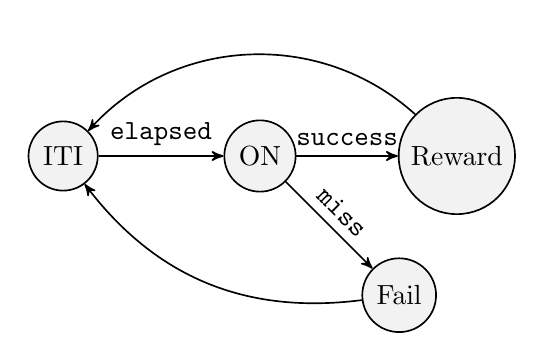
\begin{tikzpicture}
  \node[state] (iti) {ITI};
  \node[state, right of=iti] (stim) {ON};
  \node[state, right of=stim] (succ) {Reward};
  \node[state, below right of=stim] (fail) {Fail};
  \draw (iti) edge node {\tt elapsed} (stim);
  \draw (stim) edge node[sloped] {\tt success} (succ);
  \draw (stim) edge node[sloped] {\tt miss} (fail);
  \draw (succ) edge[bend right=45] (iti);
  \draw (fail) edge[bend left] (iti);
\end{tikzpicture}

\end{document}